\setcounter{page}{1}
\section*{Zielsetzung}
In dem Versuch V47 wird die Molwärme von Kupfer $\ce{Cu}$ bestimt werden.
Molwärme wird hierbei als Synonym für die \emph{molare Wärmekapazität} verwendet.
Diese gibt die Menge an Wärme an, die benötigt ist um $\SI{1}{\mol}$ eines Stoffes
bzw. Elements um einen $\SI{1}{\kelvin}$ zu erwärmen.

\section{Theorie}
Im Folgenden werden drei Methodiken zur Bestimmung der Molwärme erläutert.
Zunächst wird die Molwärme klassisch hergeleitet. Anschließend werden zwei
quantenmechanische Modelle von \emph{Einstein} und \emph{Debye}
vorgestellt. Hierfür werden die Quellen \cite{anleitungV47} und \cite[S. 215]{marx} verwendet.

Weiterhin kann die Molwärme bei unterschiedlichen Bedingungen betrachtet werden.
Wird der äußere Druck $p$ festgehalten, wird von der Wärmekapazität bei konstantem
Druck gesprochen. Aus der Thermodynamik folgt für diesen Fall der Zusammenhang:
\begin{equation}
  \label{eq:C_P}
  C\ua{p} = \left.\frac{\partial Q}{\partial T}\right|_{\map{p}}.
\end{equation}
Anstatt des Druckes $p$ kann auch das Volumen des Festkörpers $V$ festgehalten
werden. Dies definiert die Wärmekapazität bei konstantem Volumen:
\begin{equation}
  \label{eq:C_V}
  C\ua{V} = \left.\frac{\partial Q}{\partial T}\right|_{V} = \left. \frac{\partial U}{\partial T}\right|_{V}.
\end{equation}
Auf Grund der Tatsache das sich $C\ua{V}$ aus der inneren Energie $U$ ableiten
lässt, ist die Beschreibung über ein theoretisches Modell leichter zu realisieren.
Jedoch kann in einem Experiment kaum sichergestellt werden, dass das Volumen einer
Probe konstant bleibt. Aus diesem Grund wird meist $C_p$ gemssen und mit Hilfe
der folgenden Formel
\begin{equation}
  \label{eq:Umrechnung_CP_CV}
  C\ua{p} - C\ua{V} = 9\alpha^2 \kappa V_0 T
\end{equation}
umgerechnet werden. Die in der Gleichun \eqref{eq:Umrechnung_CP_CV} auftretenden
Größen sind - der lineare Ausdehungskoeffizient $\alpha$, das Kompressionsmodul
$\kappa$ und das Molvolumen $V_0$.
\subsection{Klassische Betrachtung}
Klassisch lässt sich die mittlere freie innere Energie $\left<U\right>$ aus dem
\emph{Äquipartitionstheorem} ableiten. Dieses besagt, dass auf jeden quadratischen
Freiheitsgrad eine mittlere Energie von $\frac{1}{2}\map{k_B}T$ entfällt.
Für ein einzelnes Atom ergibt sich somit aus der kinetischen Energie $\frac{1}{2}mv_i^2$ und
dem quadratischen Potential der Gittschwingung $\frac{1}{2}kx_i^2$:
\begin{equation}
  \label{eq:innere_Energie}
  \left<U\,\right> = \underbrace{3}_{\map{Raumrichtungen}}\map{k_B}T.
\end{equation}
Für die innere Energie pro $\si{mol}$ ergibt sich mit der Avogradokonstante
$\map{N_A}$ folglich:
\begin{equation}
  \label{eq:klassische_innere_Energie}
  \left<U\,\right> = 3\underbrace{\map{N_A} \map{k_B}}_{=\map{R}} T.
\end{equation}
Aus der Gleichung \eqref{eq:klassische_innere_Energie} lässt sich das
\emph{Dulong-Petische Gesetz} ableiten:
\begin{equation}
  \label{eq:dulong_petit}
  C\ua{V}=\left. \frac{\partial U}{\partial T}\right|_{V}=3R
\end{equation}
Nach dem Dulong-Petischen Gesetz ist die Wärmekapazität, jedoch Material und
Temperaturunabhängig. Im späteren Verlauf werden wir zeigen, dass das Dulong-Petische Gesetz
im Grenzfall aus den quantenmechanischen Theorien folgt.

\subsection{Quantenmechanische Betrachtung}
Die bisherige klassiche Betrachtungsweise der inneren Energie, hat die
Quantisierung der Gitterschwingung noch nicht berücksichtigt.
Gitterschwinugngen lassen sich als Oszillatoren vereinfacht darstellen. Für diese
sind die zugehörigen Eigenenergien gegebn durch
\begin{equation}
  \label{eq:energie_quanten_oszi}
  E_n = \hbar \omega \left(n + \frac{1}{2}\right).
\end{equation}
Über die Zustandssumme des quantenmechanischen Systems lässt sich die innere Energie
für $3N$ harmonische Oszillatoren wie folgt berechnen:
\begin{equation}
  \label{eq:innere_energie}
  \left<U\right> = -3N\frac{1}{Z}\partial_\beta Z, \quad \text{mit} \quad \beta = \frac{1}{\map{k_B}T}
\end{equation}
Hierbei ist die Zustandsumme für die obige Energie (vgl. Gleichung \eqref{eq:energie_quanten_oszi})
gegeben als
\begin{equation}
  \label{eq:Zustandsumme}
  Z = \sum_n^\infty \exp\left(-\beta\hbar\omega\left(n+\frac{1}{2}\right)\right).
\end{equation}
Wird die Zustandsumme \eqref{eq:Zustandsumme} in die Gleichung \eqref{eq:innere_energie}
eingesetzt folgt:
\begin{equation*}
  \left<U\right>= 3N  \frac{ \sum_n^\infty \hbar\omega\left( n+ \frac{1}{2} \right)\exp\left(-\beta\hbar\omega\left( n+\frac{1}{2} \right) \right) }{ \sum_n^\infty \exp\left( -\beta\hbar\omega\left( n+\frac{1}{2} \right) \right)}.
\end{equation*}
Nach einigen Umformungsschritten - nachlesbar in Quelle \cite[S. 220]{marx} folgt für die innere Energie:
\begin{equation}
  \label{eq:innere_Energie_Quantenmechanik_diskrete}
  \left<U\right> = 3N\hbar\omega\left(\frac{1}{2} + \frac{1}{\exp\left(\hbar\omega\beta\right) -1}\right).
\end{equation}
Hierbei ist $\frac{1}{\exp\left(\hbar\omega\beta\right) -1}$ die \emph{Bose-Einstein Statistik}.

\subsubsection{Einstein-Modell}
Das von Albert Einstein im Jahre 1907 formulierte Modell nimmt eine konstante
Dispersionrelation für alle $3N$ Eigenschwingung an:
\begin{equation}
  \label{eq:dispersion_einstein}
  \omega=\omega\ua{E}=\map{const}.
\end{equation}
Für die Wärmekapazität folgt somit mit Gleichung \eqref{eq:innere_Energie_Quantenmechanik_diskrete}:
\begin{equation}
  \label{eq:CV_einstein}
  C\ua{V}^{\map{E}}= 3N\map{k_B}\left(\frac{\Theta\ua{E}}{T}\right)^2\frac{\exp\left(\frac{\Theta\ua{E}}{T}\right)}{\left(\frac{\Theta\ua{E}}{T}-1\right)^2}, \quad \text{mit} \quad \Theta\ua{E} = \frac{\hbar\omega\ua{E}}{\map{k_B}}
\end{equation}
Wird die Approximation \eqref{eq:CV_einstein} für hohe und niedrige Temperatruen
betrachtet, folgt:
\begin{equation}
  C\ua{V}^{\map{E}}=
  \begin{cases}
     3N\map{k_B}\left(\frac{\Theta\ua{E}}{T}\right)^2 \exp\left(-\frac{\Theta\ua{E}}{T}\right), &\text{für } T\ll\Theta\ua{E}  \\
     3N\map{k_B}, & \text{für } T \gg \Theta\ua{E}
  \end{cases}
\end{equation}
Bei der Betrachtung der Anzahl der Atome pro $\si{mol}$ kann $N$ durch $\map{N_A}$
ersetzt werden und es ergibt sich das in \eqref{eq:dulong_petit} definierte
Dulong-Petische Gesetz. In der Abbildung \ref{fig: einstein_modell_plot} ist zu erkennen, wie das Einstein-Modell
experimentelle Daten beschreibt.
\begin{figure}
  \centering
  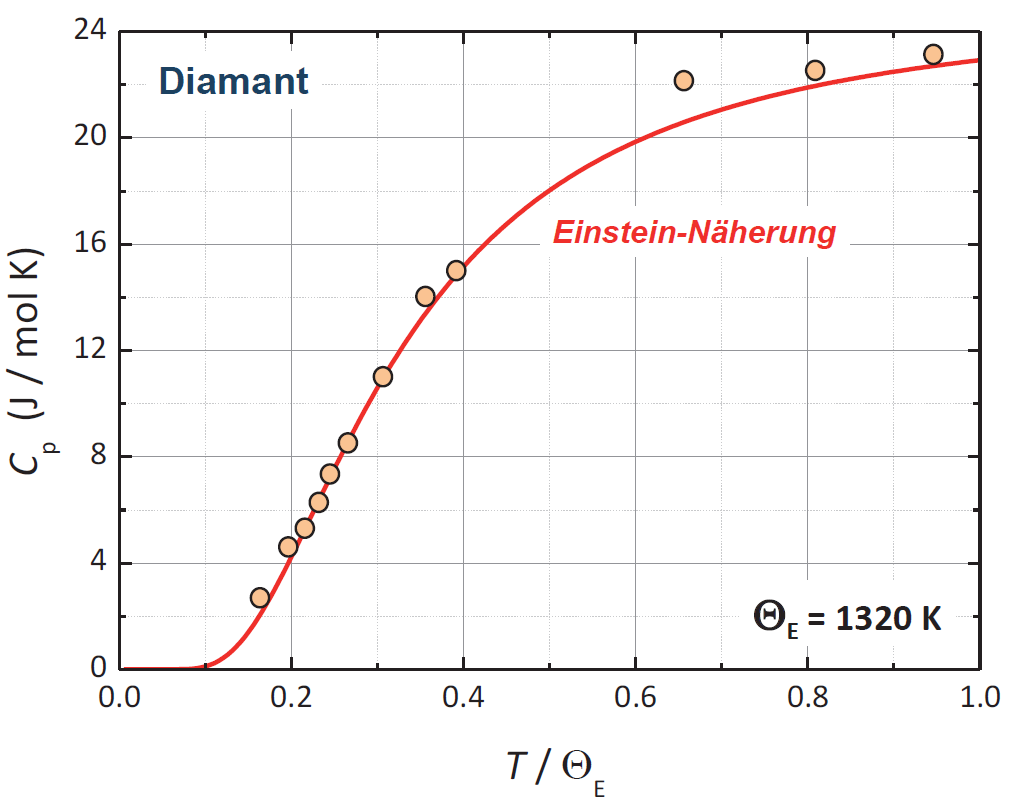
\includegraphics[width = 0.65\textwidth]{./content/images/einstein.PNG}
  \caption{Die experimentell Bestimmte molare Wärmekapazität von Diamant. Zusätzlich ist die durch das Einstein-Modell
  gegebene theoretische Beschreibung mit eigezeichnet \cite[S. 225]{marx}.}
  \label{fig: einstein_modell_plot}
\end{figure}
Das Einstein-Modell eignet sich sich gut, wenn optische Phononen dominieren oder eine
flache Dispersionsrelation vorligen (vgl. Abbildung \ref{fig: dispersions_relation}).
\begin{figure}
  \centering
  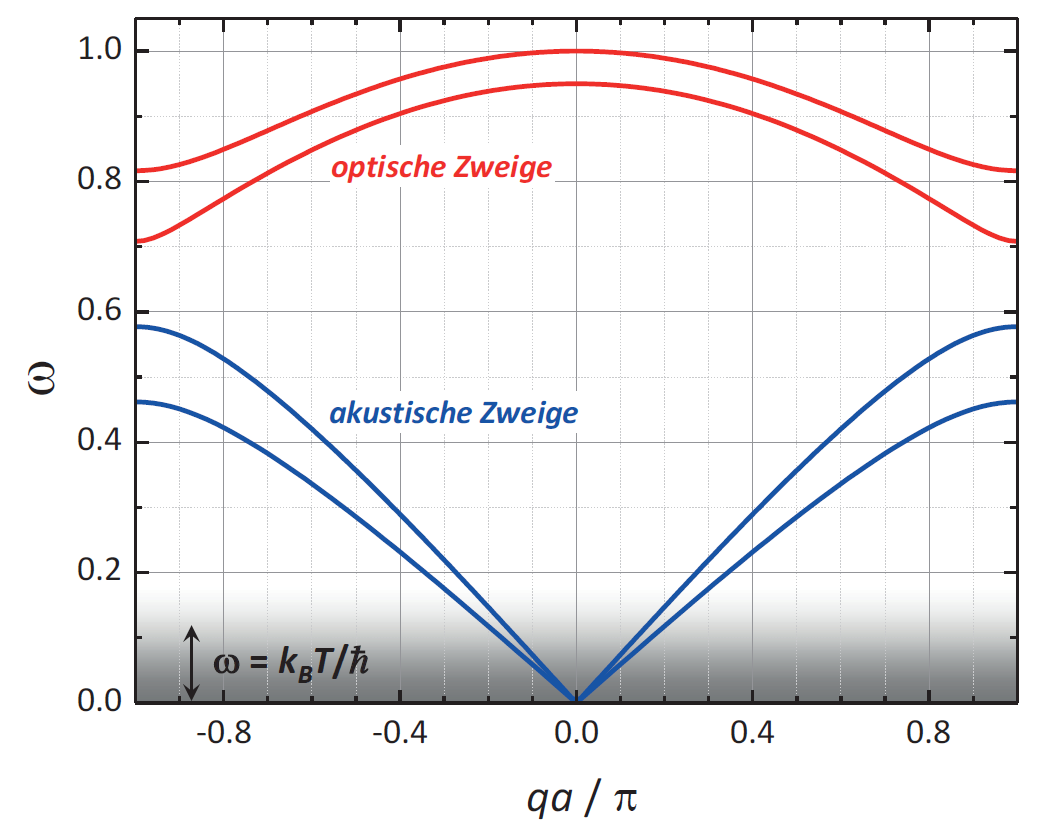
\includegraphics[width = 0.65\textwidth]{./content/images/optische_akustische.PNG}
  \caption{Schematische Darstellung von optischen und akustischen Dispersionszweigen \cite[S. 223]{marx}.}
  \label{fig: dispersions_relation}
\end{figure}
Zusätzlich ist in der Abbildung \ref{fig: dispersions_relation} deutlich zu erkennen,
das akustische Phonen um $0$ eine annähernd lineare Dispersionsrealtion aufweist.
Dies ist die Motivation für das zweite quantenmechanische Modell, das
Debye-Modell.

\subsubsection{Debye-Modell}
